% !TeX encoding = UTF-8
% 主文件--main.tex
\documentclass[
	type = bachelor,	% bachelor | master | doctor
	%submit,
	%openany,			% openany | openright(default)
	fontset = windows,  % fandol | windows (normal)
]{buctthesis}

% 在这个文件里载入其他对写作有帮助的宏包,或自定义命令等
\usepackage{mycfg}

\buctsetup{
	% 论文的中文标题
	ChineseTitle		= {基于 \LaTeX\ 的北京化工大学本硕博毕业论文写作模板},
	% 封面上的标题。总字数不要超过 36 个汉字长度。
	% 本科:可以一行或分两行写,如无第二行将 ChineseTitleLineB 留空或注释掉;
	% 封面标题首行
	ChineseTitleLineA	= {基于 \LaTeX\ 的北京化工大学本硕博},
	% 封面标题次行
	ChineseTitleLineB	= {毕业论文写作模板},
	% 论文的英文标题,一般需要大写
	EnglishTitle		= {BUCTthesis: A \LaTeX\ WRITING TEMPLATE FOR BUCT},
	% 作者的中文姓名
	author				= {张三},
	% 班级(仅本科)
	class				= {某某1024},
	% 学号
	studentid			= {2018020999},
	% 学院(仅本科)
	school				= {材料科学与工程学院},
	% 专业名称(仅本科)
	major				= {高分子材料与工程},
	% 导师的姓名与职称(仅本科)
	supervisor			= {李四教授},
	% 专业负责人姓名(仅本科)
	msupervisor			= {王五},
	% 中文、英文关键词,各关键词间以西文逗号“,”分隔
	ChineseKeywords		= {论文,\LaTeX{},模板},
	EnglishKeywords		= {thesis,\LaTeX{},template},
	% 日期,请注意:务必使用形如“YYYY-MM-DD”的格式
	date				= {2023-05-20},
}

\begin{document}
	% 生成封面,请确保字体文件的存在
	\makecover
	
	% 从此以大写罗马数字编页码
	\frontmatter
	
	% 诚信声明、任务书、摘要
	%% 前置部分--frontmatter.tex
%% 诚信声明
\makedeclare%[figure/declare-master-doctor.png]

%% 摘要
\begin{cabstract}
	摘要和关键词一起写在这里。

	摘要是学位论文的内容不加注释和评论的简短陈述,置于学位论文数据集后。
	摘要应具有独立性和自含性,即不阅读论文的全文,
	就能获得必要的信息。摘要中有数据、结论,是一篇完整的短文,
	可以独立使用和引用。摘要的内容应包含与论文正文等同量的主
	要信息,供读者确定有无必要阅读全文,也可供二次文献(文摘
	等)采用。摘要一般应说明研究工作的目的、实验方法、结果和
	最终结论等,重点突出具有创新性的成果和新见解。
	
	硕士论文摘要 500 字左右,博士论文摘要 1500 字左右。
	英文摘要应与中文摘要内容一致。除无法变通的办法可用以外,
	摘要中不用图、表、化学结构式、非公知公用的符号和术语。
	
	接下来的一大段废段话的作用是将中文摘要写到 1500 个字。
	
	\zhlipsum[1-3]
	
	本项目的创新点有:
	\begin{enumerate}
		\item 开发了第一份适用于北京化工大学毕业论文的 \LaTeX\ 模板;
		\item 以自身为示例展示此模板的使用方法;
		\item 这是编号列表环境的第三项。
	\end{enumerate}

	(以上共约 1600 字)
\end{cabstract}

\begin{eabstract}
	Here is the Abstract and the Keywords.

	The followings are nonsense.

	\lipsum[1-7]

	Innovations in the research:
	\begin{itemize}
		\item Developing the first \LaTeX{} writting template for BUCT undergraduate thesis;
		\item Using the PDF itself as an example to show how to use the template;
		\item This is the third item of an unnumbered list.
	\end{itemize}

	(Around 5000 letters above)
\end{eabstract}
	
	% 生成主目录
	\tableofcontents
	% 设计图纸目录,这与主目录独立。
	\listofdesignfigures
	
	% 前言
	%% 前言--foreword.tex
\begin{foreword}
这里是前言。点明毕业论文的论题、学术意义以及其与所阅读文献的关系,
简要说明文献收集的目的、重点、时空范围、文献种类、核心刊物等方面的内容。

豫章故郡,洪都新府。星分翼轸,地接衡庐。襟三江而带五湖,控蛮荆而引瓯越。
物华天宝,龙光射牛斗之墟;人杰地灵,徐孺下陈蕃之榻。雄州雾列,俊采星驰。
台隍枕夷夏之交,宾主尽东南之美。都督阎公之雅望,棨戟遥临;宇文新州之懿
范,襜帷暂驻。十旬休假,胜友如云;千里逢迎,高朋满座。腾蛟起凤,孟学士
之词宗;紫电青霜,王将军之武库。家君作宰,路出名区;童子何知,躬逢胜饯。

时维九月,序属三秋。潦水尽而寒潭清,烟光凝而暮山紫。俨骖騑于上路,访风
景于崇阿。临帝子之长洲,得仙人之旧馆。层峦耸翠,上出重霄;飞阁流丹,下
临无地。鹤汀凫渚,穷岛屿之萦回;桂殿兰宫,即冈峦之体势。

披绣闼,俯雕甍,山原旷其盈视,川泽纡其骇瞩。闾阎扑地,钟鸣鼎食之家;舸
舰迷津,青雀黄龙之舳。云销雨霁,彩彻区明。落霞与孤鹜齐飞,秋水共长天一
色。渔舟唱晚,响穷彭蠡之滨,雁阵惊寒,声断衡阳之浦。

遥襟甫畅,逸兴遄飞。爽籁发而清风生,纤歌凝而白云遏。睢园绿竹,气凌彭泽
之樽;邺水朱华,光照临川之笔。四美具,二难并。穷睇眄于中天,极娱游于暇
日。天高地迥,觉宇宙之无穷;兴尽悲来,识盈虚之有数。望长安于日下,目吴
会于云间。地势极而南溟深,天柱高而北辰远。关山难越,谁悲失路之人;萍水
相逢,尽是他乡之客。怀帝阍而不见,奉宣室以何年?

嗟乎!时运不齐,命途多舛。冯唐易老,李广难封。屈贾谊于长沙,非无圣主;
窜梁鸿于海曲,岂乏明时?所赖君子见机,达人知命。老当益壮,宁移白首之心?
穷且益坚,不坠青云之志。酌贪泉而觉爽,处涸辙以犹欢。北海虽赊,扶摇可接;
东隅已逝,桑榆非晚。孟尝高洁,空余报国之情;阮籍猖狂,岂效穷途之哭!

勃,三尺微命,一介书生。无路请缨,等终军之弱冠;有怀投笔,慕宗悫之长风。
舍簪笏于百龄,奉晨昏于万里。非谢家之宝树,接孟氏之芳邻。他日趋庭,叨陪
鲤对;今兹捧袂,喜托龙门。杨意不逢,抚凌云而自惜;钟期既遇,奏流水以何惭?

呜乎!胜地不常,盛筵难再;兰亭已矣,梓泽丘墟。临别赠言,幸承恩于伟饯;
登高作赋,是所望于群公。敢竭鄙怀,恭疏短引;一言均赋,四韵俱成。请洒潘
江,各倾陆海云尔:

\begin{center}
滕王高阁临江渚,佩玉鸣鸾罢歌舞。

画栋朝飞南浦云,珠帘暮卷西山雨。

闲云潭影日悠悠,物换星移几度秋。

阁中帝子今何在?槛外长江空自流。
\end{center}

\end{foreword}


	
	% 从此以阿拉伯数字编页码
	\mainmatter
	
	% 正文各章节
	%% 第一章--chapter1.tex
\chapter{绪论}
\section{字体}
\subsection{字体配置}
模板配置了两种字库,以 \opt{fontset = windows} 为例:
\begin{enumerate}
	\item 中文:主字体(衬线字体)为中易宋体,无衬线字体族为中易黑体,%
	且二者均可加粗为对应的伪粗体;《规范》中未规定的楷体和仿宋均为 \pkg{ctex} 宏集的预设,为避免格式审查问题,应当减少使用;
	\item 西文:除英文摘要的关键词使用中易黑体、除公式中的西文(数字、字母等)使用特殊字体,其它一律使用 Times New Roman;
	\item 公式:模板会根据实际字体安装情况,选择 $LibertinusMath$ 字体或使用 \LaTeX\ 的默认字体。
\end{enumerate}

\subsection{中文字体命令及对应西文示例}
\begin{enumerate}
	\item 宋体:北京化工大学 BUCT 1958 或 \textrm{北京化工大学 BUCT 1958}
	\item 粗宋体:{\bfsong 北京化工大学 BUCT 1958} 或 \emph{北京化工大学 BUCT 1958}
	\item 黑体:{\heiti 北京化工大学 BUCT 1958} 或 \textsf{北京化工大学 BUCT 1958}
	\item 粗黑体:{\bfhei 北京化工大学 BUCT 1958} 或 \textsf{\bfseries 北京化工大学 BUCT 1958}
	\item 仿宋:{\ttfamily 北京化工大学 BUCT 1958} 或 \texttt{北京化工大学 BUCT 1958}
	\item 斜体:{\itshape 北京化工大学 BUCT 1958} 或 \textit{北京化工大学 BUCT 1958}
\end{enumerate}

\section{浮动体}
% 一些文字用来充版面。摘自 https://github.com/chinese-poetry/chinese-poetry
六王毕,四海一,蜀山兀,阿房出。覆压三百余里,隔离天日。骊山北构而西折,直走咸阳。
二川溶溶,流入宫墙。五步一楼,十步一阁;廊腰缦回,檐牙高啄;各抱地势,钩心斗角。
盘盘焉,囷囷焉,蜂房水涡,矗不知其几千万落。长桥卧波,未云何龙?复道行空,不霁何虹?
高低冥迷,不知西东。歌台暖响,春光融融;舞殿冷袖,风雨凄凄。一日之内,一宫之间,而气候不齐。

妃嫔媵嫱,王子皇孙,辞楼下殿,辇来于秦,朝歌夜弦,为秦宫人。明星荧荧,开妆镜也;
绿云扰扰,梳晓鬟也;渭流涨腻,弃脂水也;烟斜雾横,焚椒兰也。雷霆乍惊,宫车过也;
辘辘远听,杳不知其所之也。一肌一容,尽态极妍,缦立远视,而望幸焉。有不见者,三十六年。
燕赵之收藏,韩魏之经营,齐楚之精英,几世几年,剽掠其人,倚叠如山。一旦不能有,输来其间。
鼎铛玉石,金块珠砾,弃掷逦迤,秦人视之,亦不甚惜。

\subsection{插图}\label{subsec:fig}

一般的图片插入使用 \env{figure} 环境。
一张普普通通的插图参见图~\ref{fig:a-single-image}。

\begin{figure}[H]
	\centering
	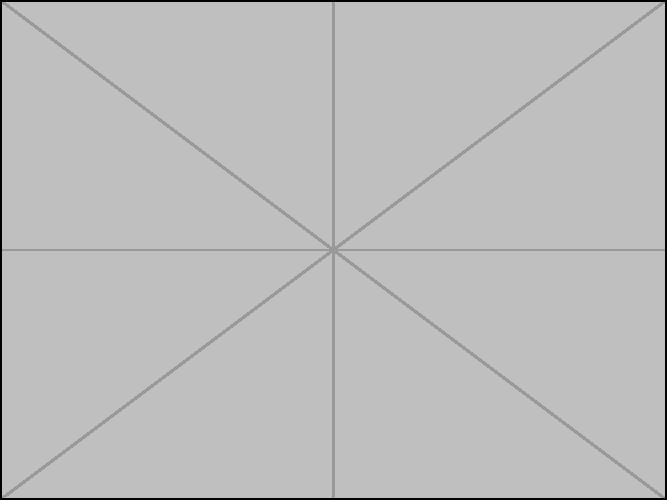
\includegraphics[width=0.3\textwidth]{image-plain.pdf}
	\caption{一张插图。加上参数 [H] 固定图片位置,禁止“浮动”}\label{fig:a-single-image}
\end{figure}

嗟乎!一人之心,千万人之心也。秦爱纷奢,人亦念其家。奈何取之尽锱铢,用之如泥沙!
使负栋之柱,多于南亩之农夫;架梁之椽,多于机上之工女;钉头磷磷,多于在庾之粟粒;
瓦缝参差,多于周身之帛缕;直栏横槛,多于九土之城郭;管弦呕哑,多于市人之言语。
使天下之人,不敢言而敢怒。独夫之心,日益骄固。戍卒叫,函谷举,楚人一炬,可怜焦土!

至于图片的并排,如果只需为组图写一个图注,可在一个 \env{figure} 环境中多次使用 \cs{includegraphics} 命令(可根据需要在插图之间加入空白)。两张并排的图片参见图~\ref{fig:abreast-image}。

\begin{figure}[htbp]
	\centering
	
\includegraphics[width=0.3\textwidth]{image-a.pdf}
	\hspace{1cm}
	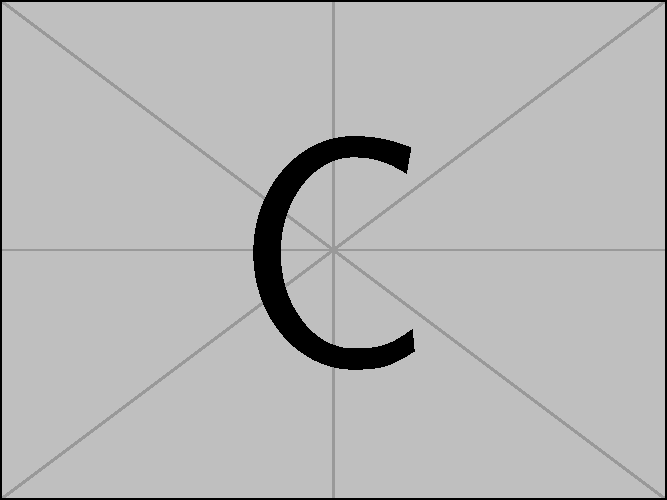
\includegraphics[width=0.3\textwidth]{image-c.pdf}
	\caption{并排的插图,这适合无需在每一张图下写图注的情况。}\label{fig:abreast-image}
\end{figure}

呜呼!灭六国者六国也,非秦也;族秦者秦也,非天下也。嗟乎!使六国各爱其人,则足以拒秦;
使秦复爱六国之人,则递三世可至万世而为君,谁得而族灭也?秦人不暇自哀,而后人哀之;
后人哀之而不鉴之,亦使后人而复哀后人也。

梁惠王曰:“寡人之于国也,尽心焉耳矣。河内凶,则移其民于河东,移其粟于河内;河东凶亦然。
察邻国之政,无如寡人之用心者。邻国之民不加少,寡人之民不加多,何也?

但如果需要在每一个子图下写上图注(或需要对子图标序),可使用 \cs{subcaptionbox} 命令。
一张子图见图~\ref{subfig:abreast-image-a},又一张子图见图~~\ref{subfig:abreast-image-c},这两张并排起来的组图见图~\ref{fig:abreast-image-a-c}。

\begin{figure}[htbp]
	\centering
	\subcaptionbox{这是一张图片。\label{subfig:abreast-image-a}}
	{
\includegraphics[height = 5cm]{image-a.pdf}}
	\hspace{1cm}
	\subcaptionbox{这又是一张图片。\label{subfig:abreast-image-c}}
	{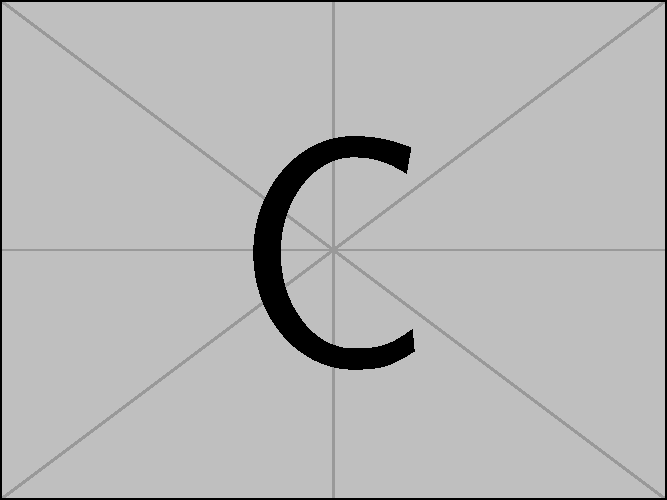
\includegraphics[angle = 90, height = 5cm]{image-c.pdf}}
	\caption{并排的插图,这适合每一张图写一个图注的情况。}\label{fig:abreast-image-a-c}
\end{figure}

孟子对曰:“王好战,请以战喻。填然鼓之,兵刃既接,弃甲曳兵而走。或百步而后止,
或五十步而后止。以五十步笑百步,则何如?”曰:“不可,直不百步耳,是亦走也。”
曰:“王如知此,则无望民之多于邻国也。不违农时,谷不可胜食也;数罟不入洿池,
鱼鳖不可胜食也;斧斤以时入山林,材木不可胜用也。谷与鱼鳖不可胜食,材木不可胜用,
是使民养生丧死无憾也。养生丧死无憾,王道之始也。五亩之宅,树之以桑,五十者可以衣帛矣
。鸡豚狗彘之畜,无失其时,七十者可以食肉矣。百亩之田,勿夺其时,数口之家,可以无饥矣;
谨庠序之教,申之以孝悌之义,颁白者不负戴于道路矣。七十者衣帛食肉,黎民不饥不寒,
然而不王者,未之有也。狗彘食人食而不知检,涂有饿莩而不知发,人死,则曰:‘非我也,
岁也。’是何异于刺人而杀之,曰‘非我也,兵也’?王无罪岁,斯天下之民至焉。”

(机械设计等)设计图纸需要编目。模板新定义了类似 \env{figure} 的 \env{dfigure}环境。
设计图纸的标签与普通插图不同,且计数器相互独立。
对于图纸的编目,可以在主文件以 \cs{listofdesignfigures} 生成独立的目录,或使用
\cs{dcaption}\marg{Caption}命令与主目录合并。
\begin{dfigure}% [H] or [htbp] is also available here.
	\centering
	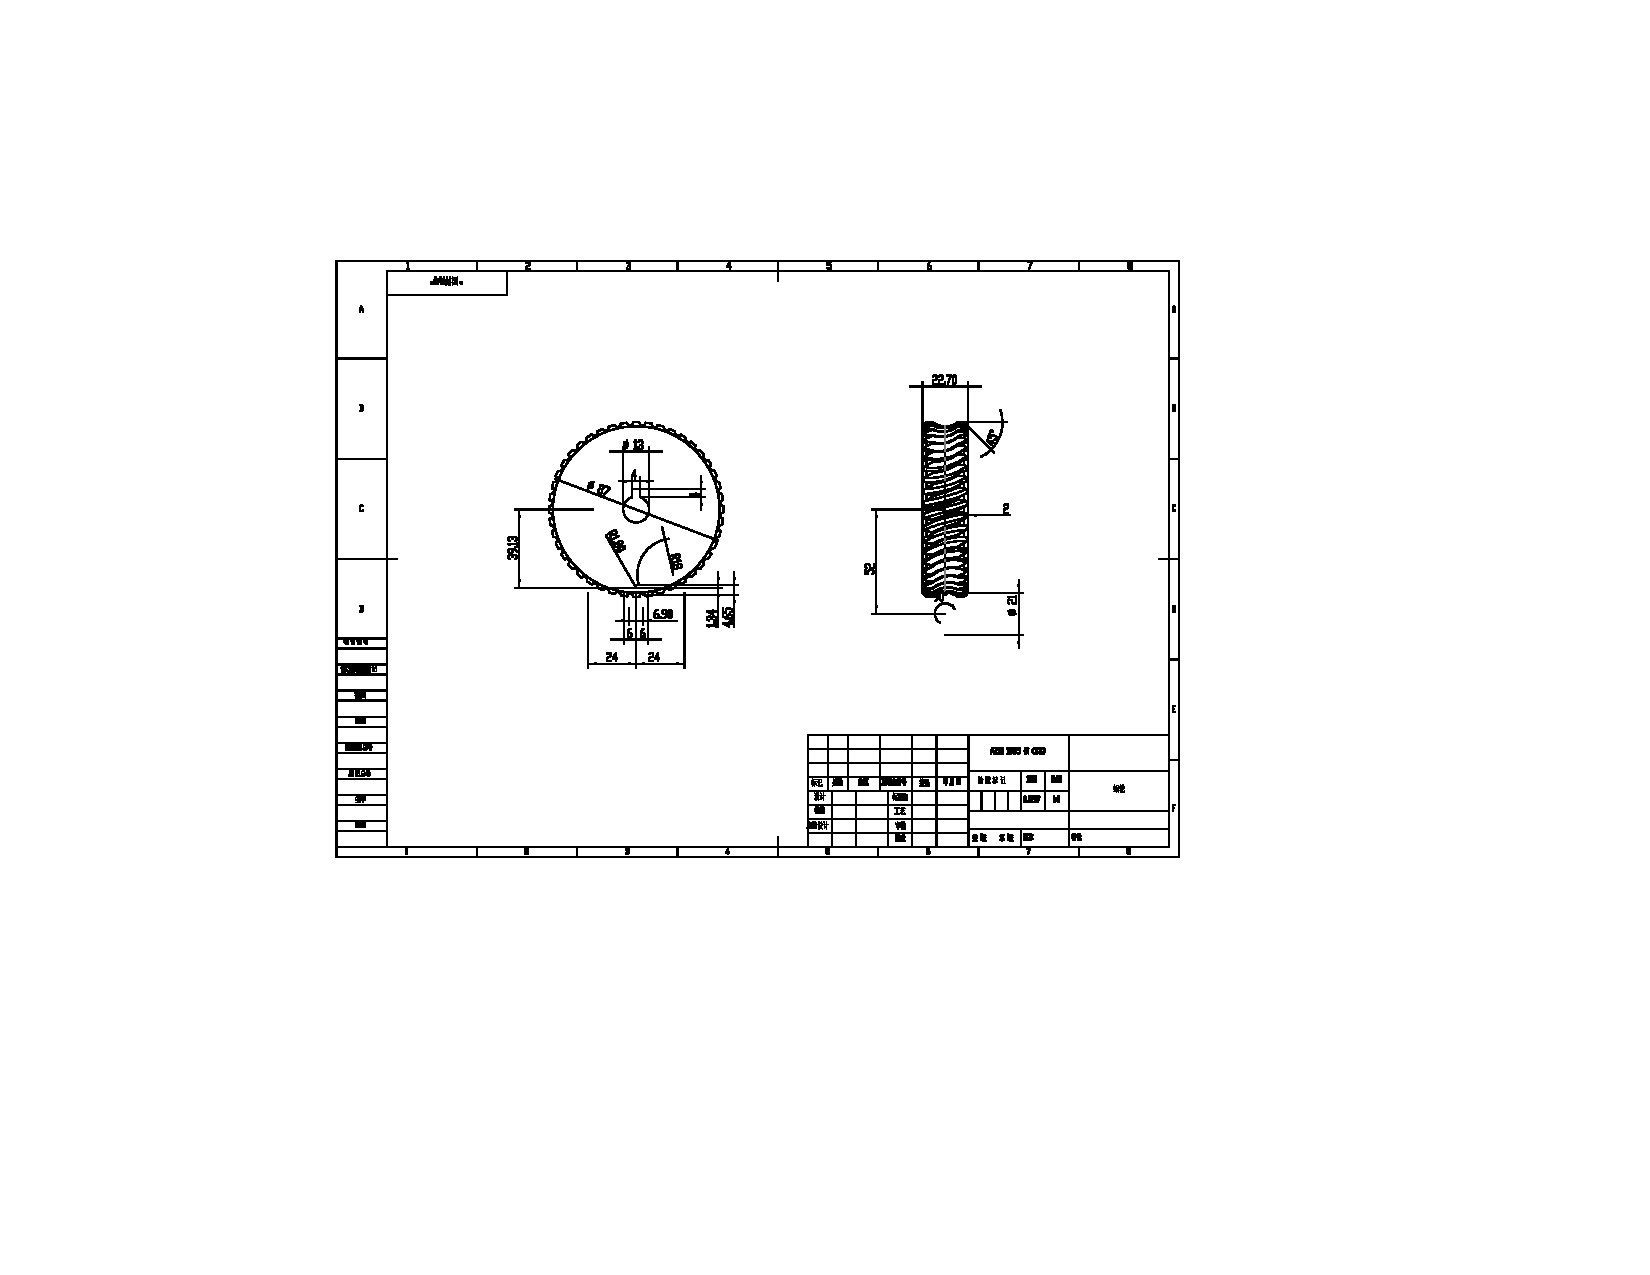
\includegraphics[width = \textwidth]{worm-gear.pdf}
	\caption{设计图纸示例}  % \dcaption{设计图纸示例} % 该命令将其编入主目录。
\end{dfigure}

以上命令适合大部分图片的插入。
但不可否认的是,\LaTeX{}对于图文混排的能力是较弱的,如果希望深入了解,推荐~
\href{https://github.com/WenboSheng/epslatex-cn}{\LaTeXe 插图指南}
(中译本第三版)作为参考资料。


\subsection{表格}\label{subsec:tab}
论文中常用三线表。本模板的组成见表~\ref{tab:mainfile}。

\begin{table}[ht]
	\centering
	\caption{模板的组成}\label{tab:mainfile}
		\begin{tabular}{ll}
			\toprule
			文件(夹)名           & 简述\\
			\midrule
			\file{chapter/}       & 论文各个部分的源文件路径\\
			\file{code/}          & 源代码的路径\\
			\file{figure/}        & 插图的路径\\
			\file{buctthesis.ins} & \textsc{DocStrip} 驱动文件\\
			\file{buctthesis.dtx} & \textsc{DocStrip} 源文件\\
			\file{main.tex}       & 主文件\\
			\file{main.pdf}       & 示例文档\\
			\file{buctthesis.cls} & 模板的文档类文件\\
			\file{thesisbib.bib}  & \BibTeX{}参考文献数据库\\
			\file{mycfg.sty}      & 自定义配置文件\\
			\file{README.md}      & 项目自述文件\\
			\file{buctthesis.pdf} & 写作指南\\
			\bottomrule
		\end{tabular}
\end{table}

北冥有鱼,其名为鲲。鲲之大,不知其几千里也。化而为鸟,其名为鹏。鹏之背,
不知其几千里也,怒而飞,其翼若垂天之云。是鸟也,海运则将徙于南冥。南冥者,
天池也。《齐谐》者,志怪者也。《谐》之言曰:“鹏之徙于南冥也,水击三千里,
抟扶摇而上者九万里,去以六月息者也。”

使用 \cs{hline}命令也能划线,但其线宽固定。关于表格内对齐与常用的命令见表~\ref{tab:tabcmd}。
\begin{table}[H]
	\centering
	\caption{表格命令举例}\label{tab:tabcmd}
	\begin{tabular}{lcrp{5em}@{\extracolsep{3em}}l}
		\hline
		左对齐 & 居中对齐 & 右对齐 & 定宽               & 增加左侧间距\\
		l     & c        &  r    & p\marg{width}  & @\{\cs{extracolsep}\marg{width}\}\\
		\hline
	\end{tabular}
\end{table}

野马也,尘埃也,生物之以息相吹也。
天之苍苍,其正色邪?其远而无所至极邪?其视下也,亦若是则已矣。且夫水之积也不厚,
则其负大舟也无力。覆杯水于坳堂之上,则芥为之舟;置杯焉则胶,水浅而舟大也。
风之积也不厚,则其负大翼也无力。故九万里,则风斯在下矣,而后乃今培风;
背负青天而莫之夭阏者,而后乃今将图南。

另外,三线表生成横线的命令 \cs{toprule}、\cs{midrule}和
\cs{bottomrule}后可以加一个可选参数来实现对线宽的控制,如果不加参数则为默认值;
而\cs{cline}可针对某些表列画上横线。
此外,两个表格也能横向并列排版,如表~\ref{tab:2tab}。

\begin{table}[H]
	\centering
	\caption{这是一个并列排版的示例}
	\label{tab:2tab}
	\begin{tabular}{|c|r|r|}
		\hline
			& \multicolumn{2}{c|}{成绩} \\\cline{2-3}
		姓名 & 语文 & 数学 \\\hline
		张三 & 91 & 92 \\\hline
		\end{tabular}
	\hspace{1cm}
	\begin{tabular}{|c|r|r|}
		\hline
		\multirow{2}*{姓名} & \multicolumn{2}{c|}{成绩} \\ \cline{2-3}
			& 语文          & 数学 \\ \hline
		李四 & 93           & 94 \\ \hline
		\end{tabular}
\end{table}

蜩与学鸠笑之曰:“我决起而飞,抢榆枋而止,时则不至,而控于地而已矣,奚以之九万里而南为?”
适莽苍者,三餐而反,腹犹果然;适百里者宿舂粮,适千里者,三月聚粮。之二虫又何知?
小知不及大知,小年不及大年。奚以知其然也?朝菌不知晦朔,蟪蛄不知春秋,此小年也。
楚之南有冥灵者,以五百岁为春,五百岁为秋。上古有大椿者,以八千岁为春,八千岁为秋。
此大年也。而彭祖乃今以久特闻,众人匹之。不亦悲乎!

至于可跨页的长表格,可以使用 \env{longtable} 来帮忙,见表~\ref{tab:longtab}。

\begin{longtable}[c]{*{5}{l}r}
	\caption{带有塑化剂的PEO-基聚合物电解质举例}\label{tab:longtab}\\
	\toprule
	\textbf{条目} & \textbf{聚合物基体} & \textbf{锂盐} & \textbf{塑化剂} & \textbf{$T$ (\si{\degreeCelsius})} & \textbf{离子电导率 (\si{S.cm^{-1}})}\\ \midrule
	\endfirsthead
	\multicolumn{6}{c}{\small 续表 \thetable\quad 带有塑化剂的PEO-基聚合物电解质举例} \\
	\toprule
	\textbf{条目} & \textbf{聚合物基体} & \textbf{锂盐} & \textbf{塑化剂} & \textbf{$T$ (\si{\degreeCelsius})} & \textbf{离子电导率 (\si{S.cm^{-1}})}\\ \midrule
	\endhead
	\bottomrule
	\endfoot\endlastfoot
	1 & PEO & LiTf & PEG & 40 & \num{e-4} \\
	2 & PEO & LiTFSI & PEGDME & 60 & \num{3.8e-4} \\
	3 & PEO & LiTf & MC3 & 25 & \num{5.0e-5} \\
	4 & PEO & LiTf & TEG & 30 & \num{6.5e-5} \\
	5 & PEO & LiTf & EC & 60 & \num{9.0e-4} \\
	6 & PEO & LiTf & PC & 60 & \num{5.2e-4} \\
	7 & PEO/P(VDF-HFP) & \ce{LiClO4} & EC/PC & 30 & \num{1.25e-3} \\
	8 & PEO/PDMAEMA & LiTFSI & Tetraglyme & 25 & \num{4.7e-4} \\
	9 & PEO & LiTf & EC & 25 & \num{1.5e-4} \\
	10 & PEO & LiTf & EC/PC & 25 & \num{1.2e-4} \\
	11 & PEO & LiTf & EC & 30 & \num{1.6e-4} \\
	12 & PEO & LiTf & LiTFSI/DEP & 20 & \num{4.6e-5} \\
	13 & PEO & \ce{LiClO4} & DOP & 25 & \num{3.8e-4} \\
	14 & PEO & \ce{LiClO4} & DBP & 25 & $\sim10^{-5}$ \\
	15 & PEO & \ce{LiClO4} & DMP & 25 & $\sim10^{-5}$ \\
	16 & PEO & LiTf & DBP & 25 & \num{6.0e-4} \\
	17 & PEO & LiTFSI & CP & 25 & $\sim10^{-5}$ \\
	18 & PEO & LiTFSI & SN & 30 & \num{1.0e-3} \\
	19 & PEO & LiTFSI & SN & 25 & \num{2.9e-3} \\
	20 & PEO & LiBOB & SN & 20 & $\sim10^{-4}$ \\
	21 & PEO & LiTFSI & BMITFSI & 25 & \num{3.2e-4} \\
	22 & PEO & LiTFSI & EMITFSI & 40 & \num{2.67e-4} \\
	23 & PEO & LiTFSI & \ce{PP13TFSI} & 40 & \num{8.93e-5} \\
	24 & PEO & LiTf & EMITf & 25 & \num{3.0e-4}\\
	25 & PEO & LiTFSI & \ce{PP13FSI} & 60 & \num{2.18e-3} \\
	26 & PEO & LiTFSI & \ce{Pyr24TFSI} & 35 & $\sim10^{-5}$ \\
	27 & PEO & \ce{LiBF4} & \ce{MMPIBF4} & 25 & \num{2.06e-3} \\
	28 & PEO & \ce{LiPF6} & \ce{MMPIPF6} & 25 & \num{1.13e-3} \\  \bottomrule
\end{longtable}

汤之问棘也是已:“穷发之北有冥海者,天池也。有鱼焉,其广数千里,未有知其修者,其名为鲲。
有鸟焉,其名为鹏。背若泰山,翼若垂天之云。抟扶摇羊角而上者九万里,绝云气,负青天,然后图南,
且适南冥也。斥鷃笑之曰:‘彼且奚适也?我腾跃而上,不过数仞而下,翱翔蓬蒿之间,此亦飞之至也。
而彼且奚适也?’”此小大之辩也。


如果希望单元格内自动换行以适应列宽,
可以使用\env{tabularx}环境,表 \ref{tab:tabularx} 是一个示例。
\begin{table}[htbp]
	\centering
	\begin{minipage}{0.9\textwidth}
		\caption{表格控制列宽及自动折行。有些时候标题会比较长,那么我们可以把表格放到一个小页环境里,从而达到比较好的折行效果。}
		\label{tab:tabularx}
		% 整张表格最大宽度设为文本宽度(由于处于小页,则为0.8倍论文文本宽度);
		% 控制第一、二列列宽,第三列允许折行
		\begin{tabularx}{\textwidth}{p{4em}p{7.5em}X}
			\toprule
									& \multicolumn{1}{c}{\em 原文}         & \multicolumn{1}{c}{\em 翻译}                                                                                         \\
			\cmidrule(l){2-3}
									& 亦余心之所善兮,虽九死其犹未悔。 & For the ideal that I hold dear to my heart,I will not regret a thousand times to die.                           \\
			\cmidrule(l){2-3}
			\multirow{3}{*}{古文翻译} & 不畏浮云遮望眼,自缘身在最高层。 & We have no fear of the clouds that may block our sights as we are already at the top of the height.              \\
			\cmidrule(l){2-3}
									& 苟利国家生死以,岂因祸福避趋之。 & I shall dedicate myself to the interests of the country in life and death irrespective of personal weal and woe. \\
			\bottomrule
		\end{tabularx}
	\end{minipage}
\end{table}

故夫知效一官,行比一乡,德合一君,而征一国者,其自视也亦若此矣。而宋荣子
犹然笑之。且举世誉之而不加劝,举世非之而不加沮,定乎内外之分,辩乎荣辱之
境,斯已矣。彼其于世,未数数然也。虽然,犹有未树也。夫列子御风而行,泠然
善也。旬有五日而后反。彼于致福者,未数数然也。此虽免乎行,犹有所待者也。
若夫乘天地之正,而御六气之辩,以游无穷者,彼且恶乎待哉?故曰:至人无己,
神人无功,圣人无名。

若要在表格中使用脚注,请参见第~\ref{subsec:footnote}小节。

一些在线网站如
~\href{http://www.tablesgenerator.com}{LaTeX Tables Generator}~
可以帮助制作更复杂的表格。
	%% 第二章--chapter2.tex
\chapter{示例}\label{chap:CodeIntro}
\section{公式与数学类环境}\label{subsec:eqandmath}
公式分为编号和不编号的两类。可以使用\env{equation}环境为公式编号。
\begin{equation}\label{eq:gougu}
	x_{1,2}=\frac{-b \pm \sqrt{b^2-4ac}}{2a}.
\end{equation}
加上 \cs{label},就能使用 \cs{ref}或 \cs{eqref}引用了。
代入式~\ref{eq:gougu},可解得式~\eqref{eq:gougu}。

不编号的公式使用 \env{equation*} 环境。
\begin{equation*}
	\int_{-\infty}^{+\infty}\frac{1}{\sqrt{2\uppi}\sigma}		% 直立的 π
	\mathrm{e}^{-\tfrac{(x-\mu)^2}{2\sigma^2}} \,\mathrm{d}x =1
\end{equation*}

行内公式可套以美元符号 \verb+$  $+,如 $f(x)=ax^2+bx+c$.
对于上述 \env{equation*} 环境中的公式(即行间公式),可套以双美元符号 \verb+$$  $$+
或 \verb+\[   \]+。
但是并不建议使用前者,因其在 \LaTeX\ 中并没有完整的重定义,有可能会在某些命令上失效。

关于公式的命令可以参考 \pkg{amsmath} 宏包说明文档,中译可参考 \href{http://static.latexstudio.net/article/2019/0204/amsmath-guide-zh-cn.pdf}{amsmath 包使用手册};
%除此之外可参考 \href{http://media.cism.it/attachments/ch8.pdf}{Higher Mathematics}。
还有一些在线网站,如 \href{https://latexlive.com/}{latexlive} 不仅能够即时预览,还提供了图像与手写识别系统。
以下举几个例子来展示最常见的用法:

由$\cos 2x=\cos^2x-\sin^2x$ ,	% 函数
则$\Vector{n}=a\Vector{x}+b\Vector{y}+c\Vector{z}.$	% 自定义向量,区别于\vec。见 mycfg.sty
又因$\mathcal{M}\in \mathbb{R}$,			% 字母样式
于是
\[
	\int_a^b f(t)\,\mathrm{d}t = \iint\limits_S g(x,y)\,\mathrm{d}x\mathrm{d}y
	= \iiint\nolimits_D\, \mathrm{d}h.	% 积分号及角标
\]
得
\[\lim_{n \to \infty}\sum_{i=1}^n{\frac{1}{n}}\sin\frac{k}{n}.\]	% 极限、无穷、求和
故
\begin{equation}\label{eq:res}
	\oint_{\gamma}f(z)\,\mathrm{d}z=2\uppi\symbfit{i}\sum^n_{k=1}\mathrm{I}(\gamma,a_k)\mathrm{Res}(f,a_k).
\end{equation}

若要公式多行对齐,可以使用 \env{align} 环境。下面的例子在等号处对齐:
\begin{align}
	x^2 + y^2 & = 1            \\
	x         & = \sqrt{1-y^2} \\\text{and also }
	y         & =\sqrt{1-x^2}
\end{align}
这会对每一行的公式进行编号。若在 \env{equation} 环境中嵌套 \env{aligned} 环境,加上参数[b]
可以达到多行对齐但只对最后一个式子编号的效果:
\begin{equation}
	\begin{aligned}[b]
		(a + b)^3   & = (a + b) (a + b)^2         \\
					& = (a + b)(a^2 + 2ab + b^2)  \\
					& = a^3 + 3a^2b + 3ab^2 + b^3
	\end{aligned}
\end{equation}

模板使用 \pkg{amsthm} 宏包预定义了部分与数学相关的环境,格式及编号如下:
\begin{axiom}
	这是一条axiom,使用\env{axiom}环境。
\end{axiom}
\begin{theorem}[某某定理]   % []内为可选参数
	这是一条theorem,使用\env{theorem}环境。
\end{theorem}
\begin{corollary}[一条推论]\label{cor:cor1}
	这是一条corollary,使用\env{corollary}环境。
\end{corollary}
\begin{proof}
	这是一条proof,使用\env{proof}环境。
	\[
		\Matrix{A}=\begin{bmatrix}
			a_{11} & \cdots  & a_{1n} \\
			\vdots & \ddots & \vdots \\
			0      & \cdots & a_{nn}
		\end{bmatrix}_{n\times n}
	\]

	在证明的最后一行会加上证毕符号,若其位置不合理则需加上命令 \cs{qedhere}。
	综上所述,推论 \ref{cor:cor1} 成立。
\end{proof}
\begin{remark}
	这是一条remark,使用\env{remark}环境。
\end{remark}
\begin{assumption}
	这是一条assumption,使用\env{assumption}环境。
\end{assumption}
\begin{definition}
	这是一条definition,使用\env{definition}环境。
\end{definition}
\begin{property}
	这是一条property,使用\env{property}环境。
\end{property}
\begin{proposition}
	这是一条proposition,使用\env{proposition}环境。
\end{proposition}
\begin{lemma}
	这是一条lemma,使用\env{lemma}环境。
\end{lemma}

以上是模板已经定义了的数学类环境,但也能自定义。
如:
\newtheorem{tale}{传说}[chapter]	% 计数与章编号相关
\begin{tale}[山经]	  % []内为可选参数
	精卫衔微木,将以填沧海。
\end{tale}
\begin{tale}[海经]
	刑天舞干戚,猛志固常在。
\end{tale}


\section{代码}\label{subsec:code}
若要在文中插入代码,简单的代码可以使用原文照列命令~\verb+\verb+或~\verb*@\verb*@,
比如~\verb-i++-、\verb*|int main|,二者区别在于,带*号的将展示代码中的空格。
如果插入代码块,可使用环境\env{lstlisting},且可以有如下选择:
\subsubsection{直接在 \LaTeX\ 中书写代码}
\begin{lstlisting}[language=C++,caption=Hello World!,label=code:HelloWorld]
/* Hello World C++ */
#include<iostream>
using namespace std;
/*****   main function	*****/
int main()
{
	cout<<"Hello World!"<<endl;		@*//Print "Hello World!", I'm \LaTeX{}!@*
	return 0;
}
\end{lstlisting}
\subsubsection{引用代码文件}
源代码存放于 \file{code/} 文件夹里,直接调用即可。
\lstinputlisting[
	language=C++,
	caption=你好,世界!,
	label=code:HelloWorld2
]{code/helloworld.cpp}

模板按照《规范》以 Times New Roman 字体书写代码。
代码的关键字以粗体标出,而注释(西文)使用斜体。
模板载入文档类时的 \opt{submit} 选项将关闭代码颜色。

代码 \ref{code:HelloWorld} 展示了如何从代码块中临时返回到 \LaTeX\ 中。

\section{化学类}
模板加载了 \pkg{mhchem} 宏包,方便了化学(方程)式的书写。
使用命令 \cs{ce}\marg{formula} 把化学(方程)式括起来。
\subsubsection{简单化学式}
\begin{table}[H]
	\centering
	\begin{tabular}{llllll}
		\ce{H2O}    & \ce{Sb2O3}  & \ce{KCr(SO4)2.12H2O} & \ce{CrO4^2-}                & \ce{[AgCl2]-}              & \ce{^{0}_{-1}M^{-}} \\
		\ce{$n$H2O} & \ce{H2(aq)} & \ce{KCr(SO4)2*12H2O} & \ce{Fe(CN)_{$\frac{6}{2}$}} & \ce{$cis${-}[PtCl2(NH3)2]} & \ce{\alpha-Al2O3}   \\
	\end{tabular}
\end{table}
\subsubsection{含键化学式}
\begin{table}[H]
	\centering
	\begin{tabular}{llll}
		\ce{A-B=C#D}                           & \ce{A\bond{-}B\bond{=}C\bond{#}D} & \ce{A\bond{1}B\bond{2}C\bond{3}D} & \ce{A\bond{~}B\bond{~-}C} \\
		\ce{A\bond{~--}B\bond{~=}C\bond{-~-}D} & \ce{A\bond{...}B\bond{....}C}     & \ce{A\bond{->}B\bond{<-}C}        &                           \\
	\end{tabular}
\end{table}
\subsubsection{化学方程式}
\begin{table}[H]
	\centering
	\begin{tabular}{llll}
		\ce{A ->[H2O] B} & \ce{A <=>[{上方文字}][{text below}] B} & \ce{A ->[$x$][$x_i$] B} & \ce{A v B (v) -> C ^ D (^)} \\
	\end{tabular}
\end{table}
\subsubsection{其他}
\begin{itemize}
	\item 标注(可能对 CJK 文字不支持):
			\ce{Zn^2+
			<=>[+ 2OH-][+ 2H+]
			$\underset{\text{amphoteres Hydroxid}}{\ce{Zn(OH)2 v}}$
			<=>[+ 2OH-][+ 2H+]
			$\underset{\text{Hydroxozikat}}{\ce{[Zn(OH)4]^2-}}$
			}
	\item 对于化学方程式等的编号,与数学方程相似:
			$$\ce{2H2O ->[{electrify}] 2H2 ^ + O2 ^}$$
			\begin{equation}
					K^\ominus  = \ce{\frac{[Hg^2+][Hg]}{[Hg2^2+]}}
			\end{equation}
\end{itemize}

至于有机化学的结构式等,尽管有一些宏包可以绘制,但使用图片插入可能是一个更好
的选择。

\section{文献引用和参考文献}\label{sec:bib}
模板使用 \cs{cite}\marg{CiteKey}命令实现上标、方括号以“顺序编码制”引用参考文献,
这是学校《规范》的要求。一个例子。\cite{abbott2016observation}而使用
\cs{nocite}\marg{CiteKey}命令则指明不引用但需要列出的参考文献。\nocite{*}

同一处引用多个文献时,应将各篇文献的引用标签一同写在 \cs{cite} 命令中,
并以西文逗号“,”分隔各标签。所产生的样式为:当在同一处引用两篇参考文献时,
引用序号将以西文逗号分隔;
当多余两篇且连续时,将标示起止序号并以短划线相连。这\cite{texbook,latexrumen}
又是\cite{texbook,latexrumen,gbt7714-2005}一个例子。\cite{abbott2016observation,texbook,latexrumen,buctthesis}

关于 \file{thesisbib.bib} 文件的编辑,
可以使用\href{http://scholar.google.com.cn/}{谷歌学术}\footnote{亦可以访问国内镜像站。}%
或\href{http://xueshu.baidu.com}{百度学术}两种方式(方法类似)将文献数据导入\BibTeX{}数据库,大致方法如下:
\begin{itemize}
	\item 在搜索框中搜索题目(或作者、DOI等),确定所引用的论文后点击“引用”;并在弹出框中,单击最下方“BibTeX”的链接,如图~\ref{fig:addbib};
	\item 在弹出的网页中复制所有代码至 \file{thesisbib.bib} 文件;
	\item 在论文中使用 \cs{cite} 命令引用相应的文献。
	% 这里用了一条简单的自定义命令,用于快速插入单张图片,见 \file{mycfg.sty}文件。
	\addfig{AddBib.png}{在谷歌学术中导出参考文献的步骤}{fig:addbib}
\end{itemize}

举个例子:经过图~\ref{fig:addbib} 所示步骤后,弹出的网页文本如下:
\begin{lstlisting}
@article{abbott2016observation,
	title={Observation of gravitational waves from a binary black hole merger},
	author={Abbott, Benjamin P and Abbott, Richard and %(省略)
	},
	journal={Physical review letters},
	volume={116},
	number={6},
	pages={061102},
	year={2016},
	publisher={APS}
}
	\end{lstlisting}
将以上内容复制进 \file{thesisbib.bib},在论文中使用
\cs{cite\{abbott2016observation\}}即可引用此文献。
这里的 “abbott2016observation”是该篇参考文献的引用标签,可以修改。
再来一个\cite{ashirov2008tetramerization} ,
网络上的资源引用\cite{buctthesis},等。

\section{其他}\label{sec:other}

\subsection{脚注}\label{subsec:footnote}
本模板采用带圈数字脚注,计数跨页重置,使用命令 \cs{footnote}\marg{text}。
前方高能\footnote{我是可爱的脚注。}。

有些情况下(比如在表格环境、各种盒子内)使用 \cs{footnote}并不能正确生成脚注。
我们可以分两步进行,先使用 \cs{footnotemark}\oarg{text} 为脚注计数,
再在合适的位置用 \cs{footnotetext}\oarg{mark}\marg{text} 生成脚注。比如表~\ref{tab:ftnt1}。
\begin{table}[htb]
	\centering
	\caption{脚注示例1}
	\label{tab:ftnt1}
	\begin{tabular}{llll}
		\hline
		人之初                & 性本善 & 性相近 & 习相远 \\
		苟\footnotemark 不教 & 性乃迁 & 教之道 & 贵以专 \\
		\hline
	\end{tabular}
\end{table}
\footnotetext{苟:如果。}

利用 \pkg{threeparttable} 宏包提供的 \env{threeparttable} 环境可以实现在表格底下写脚注,见表~\ref{tab:ftnt2}。

\begin{table}[htb]
\centering
\begin{threeparttable}
	\caption{脚注示例2}\label{tab:ftnt2}
	\begin{tabular}{cccc}
		\toprule
		昔孟母	& 择邻处\tnote{*} & 子不学	& 断机杼\\
		\midrule
		窦燕山\tnote{$\dagger$}	& 有义方 & 教五子\tnote{$\ddagger$}	&名俱扬\\
		\bottomrule
	\end{tabular}
	\begin{tablenotes}\small
		\item [*] 脚注1。
		\item [$\dagger$] 脚注2。
		\item [$\ddagger$] 脚注3。
	\end{tablenotes}
\end{threeparttable}
\end{table}

\subsection{列表环境}\label{subsec:items}
本模板提供了三种列表环境:不编号的\env{itemize}、编号的\env{enumerate}
和使用关键字的\env{description}环境。在文档的中英文摘要部分分别展示了
基础的编号和不编号的列表环境;上面三种列表环境可以嵌套使用(至多四层),
且会自动处理不同层次的缩进和编号,如下所示:
\begin{itemize}
	\item 一条
	\item 次条
	\item 这一条可以分为\dots
		\begin{itemize}
			\item 子一条
		\end{itemize}
\end{itemize}
稍复杂一点的,如:
\begin{enumerate}
	\item 中文
		\begin{description}
			\item[文言文] 古代汉语
			\item[白话文] 现代汉语
				\begin{enumerate}
					\item 口语
						\begin{enumerate}
							\item 普通话
							\item 方言
						\end{enumerate}
					\item 书面语
				\end{enumerate}
		\end{description}
	\item English
\end{enumerate}

注意:一级编号列表环境最多罗列10条,否则标签会显示错误。
%,到第11条时,标签将从第10条的\ding{201}到第11条的\ding{202}

	%% 第三章--chapter3.tex
\chapter[含 English 的标题]{这是题目含有 English 的一章,用这个例子来说明虽然章节名很长,但是可以使用简短的编目}
\section[同理节亦然]{含有English的一节}
文字words
	
	% 结论
	%% 结论--conclusion.tex
\begin{conclusion}
	这里是结论。

	对全文做出简明扼要的总结,获得的主要研究进展及结论。

	Happy \TeX ing!祝大家一切顺利!

\end{conclusion}
	
	% 参考文献。
	% 注意:至少引用一篇参考文献,否则执行全编译时下面两行会引起编译错误。
	\bibliographystyle{gbt7714-numerical}
	\bibliography{thesisbib.bib}
	
	% 符号说明
	%% 符号说明--denotation.tex
\begin{denotation}[11cm]\label{chap*:deno}%
	$\uppi$				& 圆周率			\\	
	$c_0$				& 真空中光速		\\
	$G$					& 万有引力常量	  \\
	$k$					& 静电力常量		\\
	$\varepsilon _0$	& 真空电容率		\\
	$\mu_0$				& 真空磁导率		\\
	PVA					& 聚乙烯醇,Polyvinyl Alcohol\\
	EDTA				& 乙二胺四乙酸,Ethylenediaminetetraacetic Acid\\
	上邪				& 上邪!我欲与君相知,长命无绝衰。
	山无陵,江水为竭。冬雷震震,夏雨雪。
	天地合,乃敢与君绝!\\
	春江花月夜			& 春江潮水连海平,海上明月共潮生。 \\
						& 滟滟随波千万里,何处春江无月明!  \\
						& 江流宛转绕芳甸,月照花林皆似霰;  \\
						& 空里流霜不觉飞,汀上白沙看不见。  \\
						& 江天一色无纤尘,皎皎空中孤月轮。  \\
						& 江畔何人初见月?江月何年初照人?  \\
						& 人生代代无穷已,江月年年望相似。  \\
						& 不知江月待何人,但见长江送流水。  \\
						& 白云一片去悠悠,青枫浦上不胜愁。  \\
						& 谁家今夜扁舟子?何处相思明月楼?  \\
						& 可怜楼上月徘徊,应照离人妆镜台。  \\
						& 玉户帘中卷不去,捣衣砧上拂还来。  \\
						& 此时相望不相闻,愿逐月华流照君。  \\
						& 鸿雁长飞光不度,鱼龙潜跃水成文。  \\
						& 昨夜闲潭梦落花,可怜春半不还家。  \\
						& 江水流春去欲尽,江潭落月复西斜。  \\
						& 斜月沉沉藏海雾,碣石潇湘无限路。  \\
						& 不知乘月几人归,落月摇情满江树。  \\
	CTAN		 		& Comprehensive \TeX\ Archive Network\\*
\end{denotation}
	
	% 翻译
	%% 翻译--translation.tex
\begin{translation}
	Battery

	电池

	電池

	バッテリー

	Батареи
\end{translation}
	
	% 致谢
	%% 致谢--acknowledgement.tex
\begin{acknowledgement}
	致谢部分。

	\dots

	%最后还要感谢 BUCTthesis 帮助我节省了论文排版的时间!
\end{acknowledgement}
	
	% 附录
	\appendix
	%% 附录第一章--app1.tex
\chapter{这里是附录}\label{app:1}
未尽事宜可将其列在附录中加以说明。论文有关的数据表、符号说明、计算程序、运行结果、
主要设备、仪器仪表的性能指标和测试分析结果、精度等均可列在附录中。
\section{附录的节}
与正文类似。
\begin{table}[ht]
	\centering
	\caption{测试表格}\label{tab:mytable}
	\begin{tabular}{cc}
		\toprule
		a & B   \\
		\midrule
		甲   & 乙丙丁 \\
		\bottomrule
	\end{tabular}
\end{table}

\subsection{附录的小节}
\zhlipsum[1][name = zhufu]

\begin{figure}[ht]
	\centering
	\begin{minipage}{0.4\textwidth}
		\centering
		
\includegraphics[height=4cm]{image-a.pdf}
		\caption{第一张图}\label{fig:test1}
	\end{minipage}
	\hspace{1cm}
	\begin{minipage}{0.4\textwidth}
		\centering
		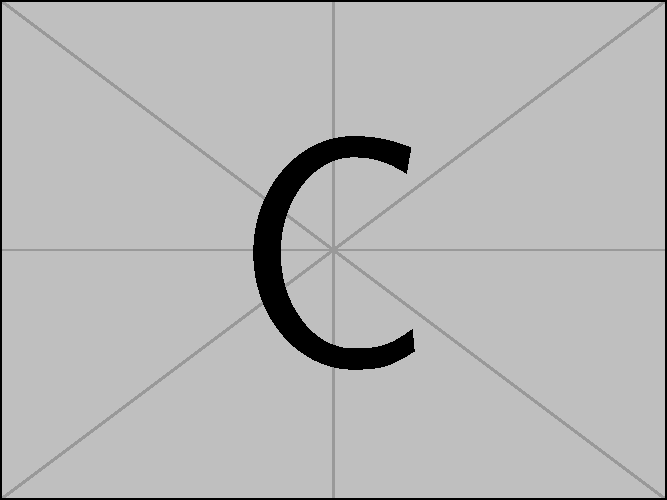
\includegraphics[height=4cm]{image-c.pdf}
		\caption{第二张图}\label{fig:test2}
	\end{minipage}
\end{figure}

\zhlipsum[name = xiangyu]

\begin{dfigure}[tbp]
	\centering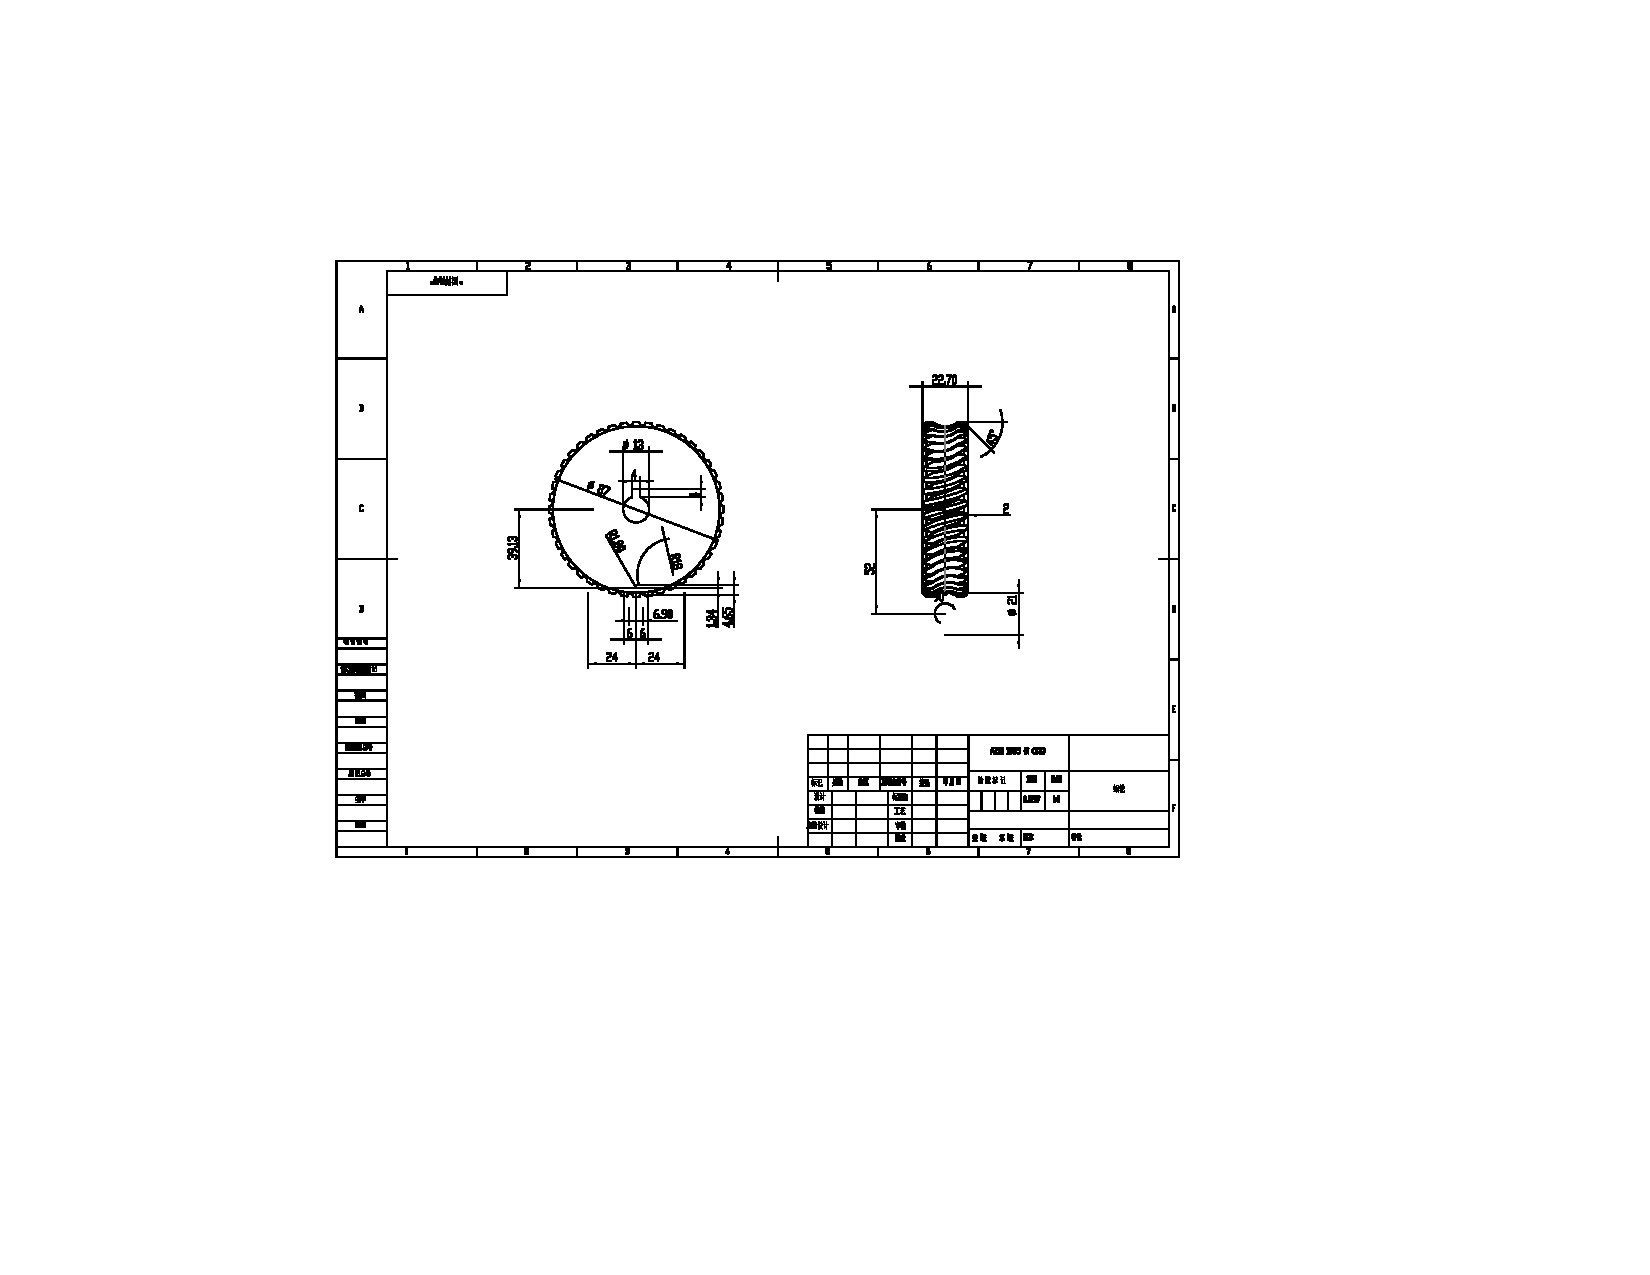
\includegraphics[height=.9\textwidth ,angle=-90]{worm-gear.pdf}
	\caption{设计图纸测试}
\end{dfigure}

\zhlipsum[1][name = aspirin]

\begin{equation}
	a^2+b^3=c^4
\end{equation}

\begin{definition}
	这是定义。\footnote{这是测试脚注。}
\end{definition}

\begin{lstlisting}[language=c++,caption=一个测试,label=mycode]
#define mian main
	\end{lstlisting}


	
\end{document}